\section{X : ADTs - Graphs}
\label{chap:adts_graphs}

%%%%%%%%%%%%%%%%%%%%%%%%%%%%%%%%%%%%%%%%%%%%%%%%%%%%%%%%%%%%%

\begin{frame}[fragile]
\frametitle{ADTs : Graphs}
\begin{columns}[T]

\begin{column}{0.45\textwidth}
\begin{itemize}[<+->]
\item A graph, $G$, consists of a set of vertices (nodes), $V$, together
with a set of edges (links), $E$, each of which connects two vertices.
\begin{center}
\includegraphics[scale=0.3]{../Images/grapha.pdf}
\end{center}
\item This is a directed graph (digraph).
Vertices are joined to adjacent vertices by these edges.
\item Every edge has a non-negative weight attached
which may correspond to time, distance, cost etc.
\end{itemize}
\end{column}

\pause
\begin{column}{0.45\textwidth}
\verb^graph.h^ (partial)
\lstinputlisting[style=basicc,linerange={7-38},numbers=none]{../../ADTs/Graph/graph.h}
\end{column}

\end{columns}
\end{frame}

%%%%%%%%%%%%%%%%%%%%%%%%%%%%%%%%%%%%%%%%%%%%%%%%%%%%%%%%%%%%%%

\begin{frame}[fragile]
\frametitle{Graph ADT : 2D Realloc I}
\begin{columns}[T]

\begin{column}{0.55\textwidth}
The graph type could be implemented in a large number
of different ways.
\begin{itemize}[<+->]
\item As two sets, one for vertices, one for edges.
We haven't looked at an implentation for sets, but one could use lists.
\item As an adjacency table - simply encode the weighted edges in a 2D array.
\begin{center}
\begin{tabular}{|c|ccccc|}\hline
& {\bf 0} & {\bf 1} & {\bf 2} & {\bf 3} & {\bf 4} \\ \hline
{\bf 0} & 0 & 5 & 3 & $\infty$ & 2 \\
{\bf 1} & $\infty$ & 0 & 2 & 6 & $\infty$ \\
{\bf 2} & $\infty$ & 1 & 0 & 2 & $\infty$ \\
{\bf 3} & $\infty$ &$\infty$ &$\infty$ & 0 & $\infty$ \\
{\bf 4} & $\infty$ & 6 & 10 & 4 & 0 \\ \hline
\end{tabular}
\end{center}
\end{itemize}
\end{column}

\pause
\begin{column}{0.35\textwidth}
\verb^specific.h^
\lstinputlisting[style=basicc]{../../ADTs/Graph/Realloc/specific.h}
\end{column}

\end{columns}
\end{frame}

%%%%%%%%%%%%%%%%%%%%%%%%%%%%%%%%%%%%%%%%%%%%%%%%%%%%%%%%%%%%%%

\begin{frame}[fragile]
\frametitle{2D Realloc II}
\begin{columns}[T]

\begin{column}{0.50\textwidth}
\lstinputlisting[style=basicc,linerange={8-40},numbers=none]{../../ADTs/Graph/Realloc/realloc.c}
\end{column}

\pause
\begin{column}{0.45\textwidth}
\lstinputlisting[style=basicc,linerange={50-79},numbers=none]{../../ADTs/Graph/Realloc/realloc.c}
\end{column}


\end{columns}
\end{frame}

%%%%%%%%%%%%%%%%%%%%%%%%%%%%%%%%%%%%%%%%%%%%%%%%%%%%%%%%%%%%%%

\begin{frame}[fragile]
\frametitle{Graph ADT - Linked}
\begin{columns}[T]

\begin{column}{0.55\textwidth}
\begin{center}
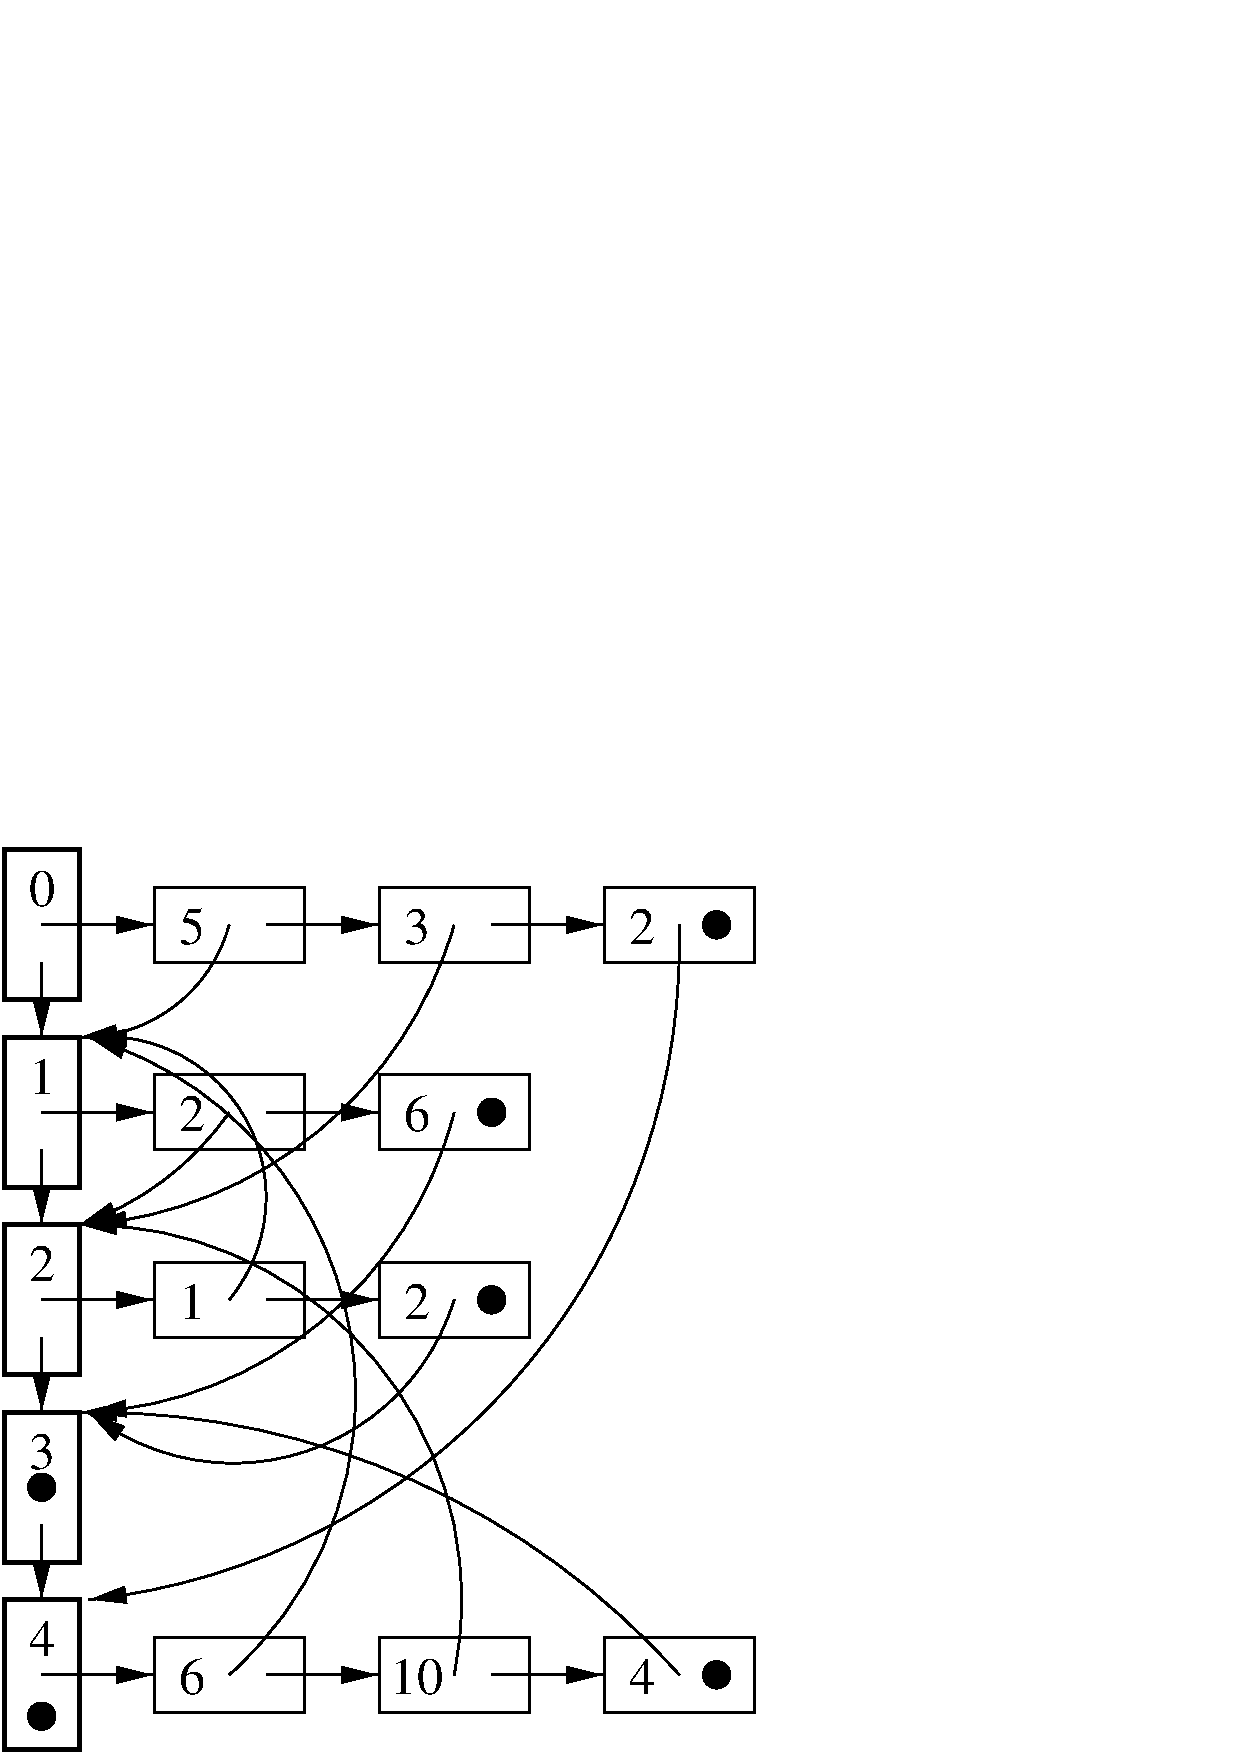
\includegraphics[height=0.75\textheight]{../Images/graphll.pdf}
\end{center}
\end{column}

\pause
\begin{column}{0.35\textwidth}
\verb^specific.h^
\lstinputlisting[style=basicc]{../../ADTs/Graph/Linked/specific.h}
\end{column}


\end{columns}
\end{frame}

%%%%%%%%%%%%%%%%%%%%%%%%%%%%%%%%%%%%%%%%%%%%%%%%%%%%%%%%%%%%%%

\begin{frame}[fragile]
\frametitle{Linked II}
\begin{columns}[T]

\begin{column}{0.45\textwidth}
\lstinputlisting[style=basicc,linerange={9-35},numbers=none]{../../ADTs/Graph/Linked/linked.c}
\end{column}

\pause
\begin{column}{0.45\textwidth}
\lstinputlisting[style=basicc,linerange={94-111},numbers=none]{../../ADTs/Graph/Linked/linked.c}
\end{column}


\end{columns}
\end{frame}
